\documentclass[11pt,a4paper,twoside,openright]{article}
\usepackage[utf8]{inputenc}
\usepackage[english]{babel} % define document language
% \usepackage{datetime}  
\usepackage[T1]{fontenc}
\usepackage{arydshln}
\usepackage{enumitem}
\usepackage{wrapfig}
\usepackage{bbold} % fct indicatrice

\usepackage{tikz}


\usepackage{url}
\usepackage[colorlinks,linkcolor=red,anchorcolor=green,citecolor=blue]{hyperref}

\usepackage{lmodern}
% \usepackage[hidelinks]{hyperref} % Hyperref package for url's and [hidelinks] option to remove collouring


\linespread{1.2}

\usepackage{amsmath,amsthm,amssymb,amsfonts}
\DeclareMathOperator*{\argmax}{arg\,max}
\DeclareMathOperator*{\argmin}{arg\,min}
\usepackage{graphicx} 
\usepackage{float} 
\usepackage{subfigure}
\usepackage{caption}
% \renewcommand{\thesubfigure}{(\roman{subfigure})}


% section title size
\usepackage{titlesec}
\titleformat*{\section}{\huge\bfseries}
\titleformat*{\subsection}{\Large\bfseries}
\titleformat*{\subsubsection}{\large\bfseries}


% \graphicspath{ {./images/} }

%marges
\usepackage{geometry}
\geometry{top= 3 cm, bottom= 3 cm, right= 2.5 cm, left= 3 cm, headheight=13.6pt}

% extra section for paragraph
\usepackage{titlesec}
\setcounter{secnumdepth}{4}
\setcounter{tocdepth}{4}
\titleformat{\paragraph}
{\normalfont\normalsize\bfseries}{\theparagraph}{1em}{}
\titlespacing*{\paragraph}
{0pt}{3.25ex plus 1ex minus .2ex}{1.5ex plus .2ex}

\newtheorem{exemple}{Exemple}

% abstract
\renewenvironment{abstract}
 {\quotation\small\noindent\rule{\linewidth}{.5pt}\par\smallskip
  {\centering\bfseries\abstractname\par}\medskip}
 {\par\noindent\rule{\linewidth}{.5pt}\endquotation}



% biblio 
\usepackage[
backend=biber,
style=alphabetic,
sorting=nyt
]{biblatex}
\usepackage{csquotes}


\usepackage[utf8]{inputenc}
\usepackage{mathrsfs}
\newtheorem{thm}{Théorème}
\newtheorem*{thm*}{Théorème}

% remarks in red
\usepackage{xcolor}
\newcommand{\rmq}[1]{\textcolor{red}{#1}}
\newcommand\ignore[1]\null

% \setcounter{secnumdepth}{0} % sections will not be enumerated

\usepackage[figurename=Fig.]{caption}
\usepackage[tablename=Tab.]{caption}


\usepackage{fancyhdr,graphicx,lastpage}% http://ctan.org/pkg/{fancyhdr,graphicx,lastpage}
\fancypagestyle{plain}{
  \fancyhf{}% Clear header/footer
  \fancyhead[R]{\textit{Internship Report}}% Right header
  \fancyhead[L]{\textit{Hrishit Tambi}}% Right header
  \fancyfoot[L]{\textit{Canopus Space}}% Left footer
  \fancyfoot[R]{\thepage\  / \pageref{LastPage}}% Right footer
}
\pagestyle{plain}% Set page style to plain.



\begin{document}
\begin{sloppypar}
\pagestyle{empty}

% Declare new goemetry for the title page only.
\newgeometry{margin=1in}
\newcommand\titleofdoc{\bfseries Internship Report}

\newcommand\GroupName{Group Name} 
\begin{titlepage}
   \begin{center}
        \vspace*{2cm} % Adjust spacings to ensure the title page is generally filled with text
        %% input logos
        {
\includegraphics[width=0.22\textwidth]{images/logo/canopus-space.jpg} \quad }

        \noindent\rule[0.25\baselineskip]{\textwidth}{1pt}
        
        \vspace{0.5 cm} 

        \Huge{\titleofdoc} 

        \vspace{0.5cm}
        \LARGE{Ship Detection in SAR images using Faster R-CNN}
          
        \vspace{2 cm}
        % \Large{\GroupName}
        \vspace{0.25cm}
        \large{\bfseries Internship carried out from March, 2023  to June, 2023}\\
        % \vfill
        \vspace{4 cm}
         
        \leftline{ \small { \textbf{Internship Mentors :} Piyush Agram, Rakesh Bhan}}

        \vspace{1 cm}
        \leftline{\small { \textbf{Company :} Canopus Space}}
        
        \noindent\rule[0.25\baselineskip]{\textwidth}{1pt}\\
    \end{center}
\setcounter{page}{0}
\end{titlepage}

\restoregeometry

% \centerline{\huge {\textbf{Acknowledgments} } }
% \setcounter{page}{-5}

% % Acknowledgments
% Say something here.


% \newpage 
% \ % The empty page
\newpage

% \section{Préambule}
\begin{abstract}
\noindent
This internship project aimed to develop a ship detection system for Synthetic Aperture Radar (SAR) images from the Capella dataset using deep learning techniques. The project utilized a Faster R-CNN model with a ResNet-50-FPN backbone, retrained on the Large-Scale SAR Ship Detection Dataset-v1.0 (LS-SSDD-v1.0). The model processes Capella Dataset images and generated a geojson file with ship detection points.

The project involved preprocessing the Capella dataset and extracting SAR images. The Faster R-CNN model was then trained, leveraging transfer learning from the ResNet-50-FPN backbone and fine-tuning on the Capella dataset. Visual analysis was also conducted to validate the detection results.

The developed ship detection system demonstrated promising performance, accurately identifying ships in SAR images and providing spatial information through the generated geojson file. The system holds potential for applications in maritime surveillance, vessel traffic monitoring, and search-and-rescue operations. \\  \\
\textit{Key words}: ship detection, SAR images, deep learning, Faster R-CNN, Capella dataset.
\end{abstract}

\newpage
\tableofcontents

\newpage
\setcounter{page}{1}
\pagestyle{plain}
\section{Importance of Ship Detection } 
Ship detection using satellite imagery is of paramount importance for several key reasons. Firstly, it plays a critical role in \textbf
{maritime surveillance}, enabling the detection of suspicious or illegal activities. By utilizing advanced image processing techniques and machine learning algorithms, satellite-based ship detection allows authorities to monitor and identify vessels involved in illicit operations such as smuggling, piracy, or unauthorized fishing.

Secondly, ship detection is crucial for \textbf{environmental monitoring}. Satellite imagery analysis helps track pollutants in the ocean, providing valuable insights into the impact of human activities on marine ecosystems. This information allows researchers and environmental agencies to take swift action in response to incidents like oil spills or chemical discharges, minimizing ecological damage and facilitating targeted mitigation efforts.

Lastly, ship detection using satellite imagery greatly enhances \textbf{search and rescue operations}. When vessels are in distress or emergencies occur at sea, quickly identifying their location is vital for timely rescue efforts. By analyzing satellite images, authorities can promptly pinpoint the position of distressed vessels, optimizing response times and maximizing the chances of successful rescues. This capability significantly contributes to saving lives and ensuring the safety of individuals at sea.

In summary, ship detection using satellite imagery serves as an indispensable tool in maritime security, environmental protection, and search and rescue operations. Its ability to detect suspicious activities, track pollutants, and aid in locating distressed vessels has far-reaching benefits across various domains, making it a crucial aspect of modern maritime operations.

\newpage
\section{Description of Dataset}
The dataset used in this project consists of Synthetic Aperture Radar (SAR) imagery sourced from the Capella dataset. SAR is a remote sensing technology that utilizes microwave signals to generate high-resolution images of the Earth's surface. One of the notable advantages of SAR is its ability to penetrate through clouds and remain unaffected by atmospheric interference. The Capella dataset comprises SAR images with a spatial resolution of 1 meter and a temporal resolution of several days. These datasets were specifically chosen based on their availability and coverage over regions with significant maritime traffic. By leveraging SAR imagery from the Capella dataset, this project obtained up-to-date and detailed information on maritime traffic in Asian countries, providing valuable insights for ship detection and analysis.

\section{Overview of Steps Involved}
Initially, the input SAR geotiff file is divided into smaller cells, which serve as the input to the detection model. Each cell undergoes normalization and transformation into tensor data, enabling it to be processed by the detection model. 
The model employs the Faster-RCNN algorithm to search for potential ship detections within each cell. When a detection is made, the x and y coordinates of the bounding box surrounding the ship are recorded. These coordinates are then converted into latitude and longitude values and added to a list of ship detections. This process enables the identification and tracking of ships within the SAR imagery.

\section{Preprocessing}
\textbf{Image Splitting}:
The SAR images were initially divided into smaller cells of size 256x256 pixels. This splitting process aids in reducing the amount of extraneous information within each image, making it easier to isolate the area of interest. By utilizing smaller cells, the subsequent analysis can focus on specific regions within the image, enhancing the efficiency and accuracy of ship detection algorithms.

\textbf{Cropping}:
Following the image splitting step, each cell underwent cropping using a bounding box generated from the pixel-wise coordinates of the cell. This cropping operation allowed us to isolate the area of interest and remove any extraneous information that lies outside the region of interest, such as areas outside of the ocean or land masses. 

By employing image splitting and cropping techniques, the preprocessing stage aims to refine the SAR images, optimizing them for subsequent ship detection algorithms and facilitating the accurate identification and analysis of ships within the maritime domain.

\newpage
\section{Overview of Faster R-CNN}
Faster R-CNN is a widely recognized object detection algorithm that has gained significant attention in recent years. It builds upon the foundation laid by the previous R-CNN and Fast R-CNN algorithms, offering improved speed and accuracy in object detection tasks.

The architecture of Faster R-CNN consists of three primary components. Firstly, the CNN backbone is a deep neural network employed to extract relevant features from the input image. These features capture important visual patterns and characteristics necessary for object detection. Secondly, the Feature Pyramid Network (FPN) generates region proposals that are likely to contain objects. This hierarchical representation enhances the detection process by incorporating multi-scale information. Lastly, the Fast R-CNN network is responsible for classifying the region proposals and refining their bounding boxes with greater precision.

In the context of ship detection, the architecture of the Faster R-CNN model has been retrained specifically on the Large-Scale SAR Ship Detection Dataset. This dataset provides an extensive collection of SAR imagery, allowing the model to learn and adapt to the unique characteristics and challenges of ship detection in SAR data.

\subsection{Transfer Learning}

In this project, we utilized transfer learning to improve the accuracy and efficiency of our ship detection algorithm. We used a pre-trained Faster R-CNN model, which was originally trained on Sentinel-1 SAR imagery, to detect ships in the Capella dataset. The pre-trained model already contains learned features and parameters that can be fine-tuned to the new dataset, reducing the amount of data needed for training and improving the model's performance. 

\begin{center}
    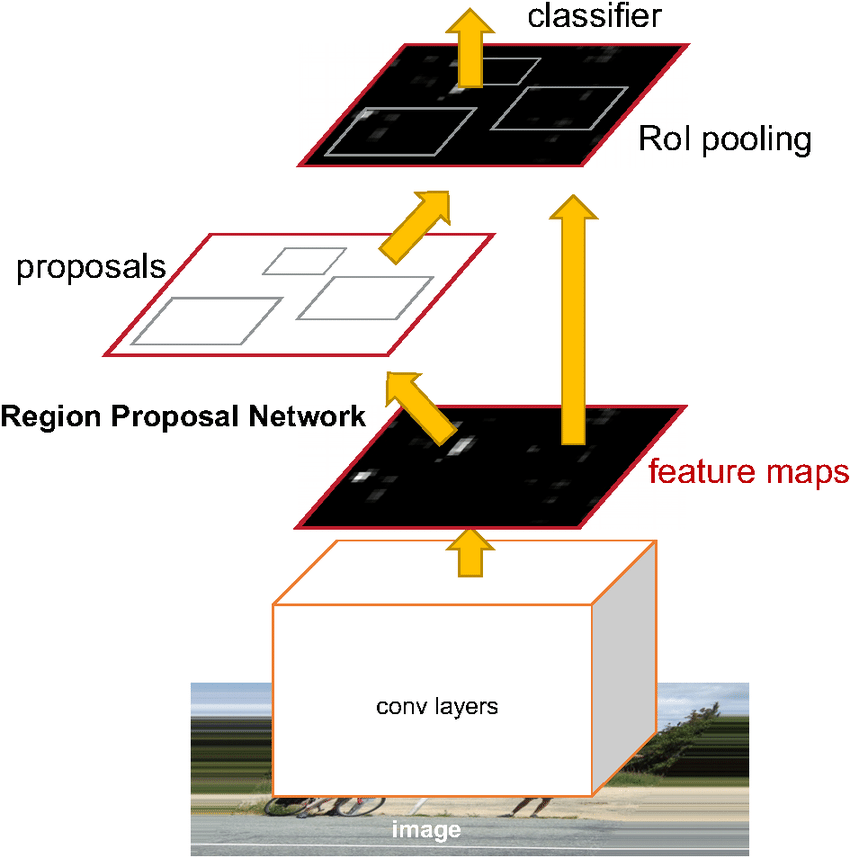
\includegraphics[scale=0.3]{images/36ba437e-08e4-4495-81e9-6487397216c7.png}   
\end{center}

\section{Conclusion}
In conclusion, deep learning approaches have shown great potential for ship detection using SAR imagery. These methods can overcome the limitations of traditional methods and achieve superior performance.
With the increasing availability of SAR data and advances in deep learning techniques, we can expect further improvements in ship detection using SAR imagery and its applications in various fields.

\end{sloppypar}
\end{document}
